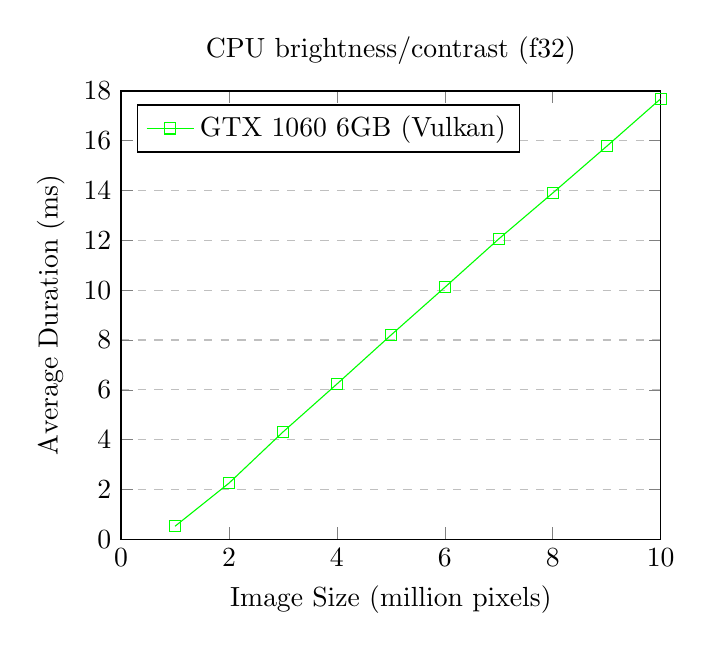
\begin{tikzpicture}
\begin{axis}[
    title={CPU brightness/contrast (f32)},
    xlabel={Image Size (million pixels)},
    ylabel={Average Duration (ms)},
    xmin=0, xmax=10,
    ymin=0, ymax=18,
    xtick={0,2,4,6,8,10},
    ytick={0,2,4,6,8,10,12,14,16,18},
    legend pos=north west,
    ymajorgrids=true,
    grid style=dashed,
]

\addplot[color=green, mark=square]
    coordinates {(1.0, 0.521246)(2.0, 2.2518999999999996)(3.0, 4.305158)(4.0, 6.231764)(5.0, 8.193256)(6.0, 10.115587)(7.0, 12.058617)(8.0, 13.902315)(9.0, 15.778357999999999)(10.0, 17.685570000000002)};
    \legend{GTX 1060 6GB (Vulkan)}

\end{axis}
\end{tikzpicture}

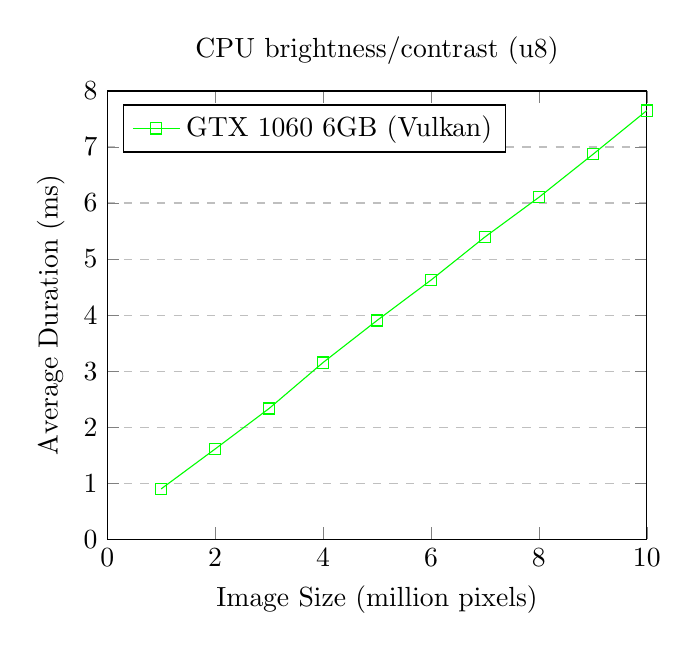
\begin{tikzpicture}
\begin{axis}[
    title={CPU brightness/contrast (u8)},
    xlabel={Image Size (million pixels)},
    ylabel={Average Duration (ms)},
    xmin=0, xmax=10,
    ymin=0, ymax=8,
    xtick={0,2,4,6,8,10},
    ytick={0,1,2,3,4,5,6,7,8},
    legend pos=north west,
    ymajorgrids=true,
    grid style=dashed,
]

\addplot[color=green, mark=square]
    coordinates {(1.0, 0.898802)(2.0, 1.610789)(3.0, 2.333491)(4.0, 3.153789)(5.0, 3.904148)(6.0, 4.624480999999999)(7.0, 5.394126)(8.0, 6.102099)(9.0, 6.868091)(10.0, 7.650309999999999)};
    \legend{GTX 1060 6GB (Vulkan)}

\end{axis}
\end{tikzpicture}

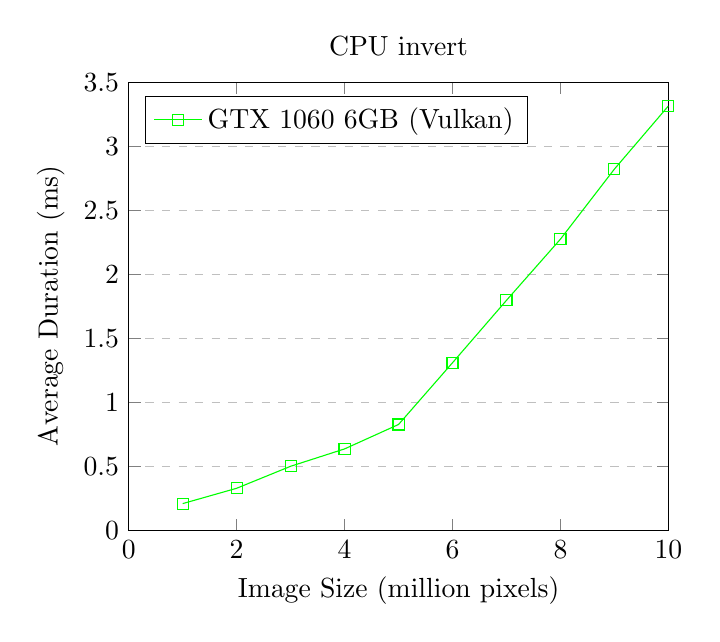
\begin{tikzpicture}
\begin{axis}[
    title={CPU invert},
    xlabel={Image Size (million pixels)},
    ylabel={Average Duration (ms)},
    xmin=0, xmax=10,
    ymin=0, ymax=3.5,
    xtick={0,2,4,6,8,10},
    ytick={0,0.5,1.0,1.5,2.0,2.5,3.0,3.5},
    legend pos=north west,
    ymajorgrids=true,
    grid style=dashed,
]

\addplot[color=green, mark=square]
    coordinates {(1.0, 0.20996099999999998)(2.0, 0.32959)(3.0, 0.5013040000000001)(4.0, 0.6369480000000001)(5.0, 0.827543)(6.0, 1.3095629999999998)(7.0, 1.796772)(8.0, 2.274414)(9.0, 2.821441)(10.0, 3.314158)};
    \legend{GTX 1060 6GB (Vulkan)}

\end{axis}
\end{tikzpicture}

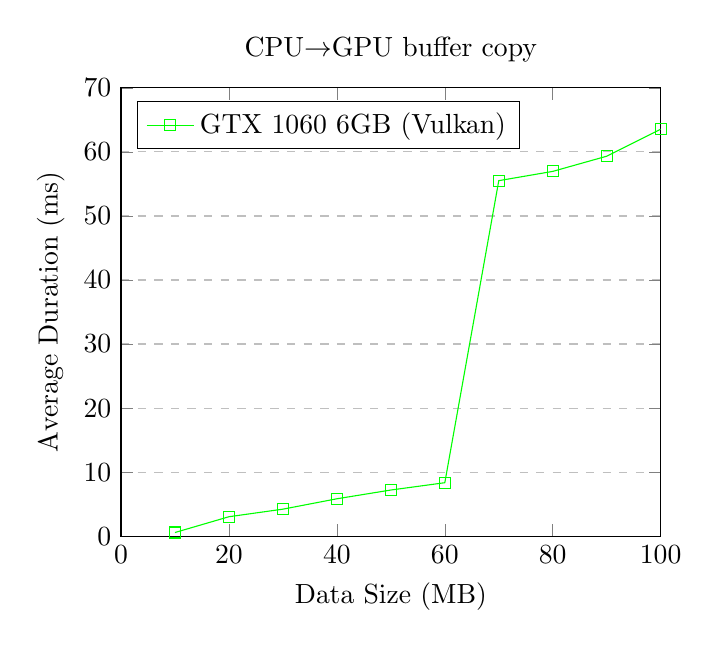
\begin{tikzpicture}
\begin{axis}[
    title={CPU$\rightarrow$GPU buffer copy},
    xlabel={Data Size (MB)},
    ylabel={Average Duration (ms)},
    xmin=0, xmax=100,
    ymin=0, ymax=70,
    xtick={0,20,40,60,80,100},
    ytick={0,10,20,30,40,50,60,70},
    legend pos=north west,
    ymajorgrids=true,
    grid style=dashed,
]

\addplot[color=green, mark=square]
    coordinates {(10.0, 0.572623)(20.0, 3.036126)(30.0, 4.218487)(40.0, 5.8384350000000005)(50.0, 7.2054279999999995)(60.0, 8.348279)(70.0, 55.511111)(80.0, 56.959264000000005)(90.0, 59.330929999999995)(100.0, 63.544306999999996)};
    \legend{GTX 1060 6GB (Vulkan)}

\end{axis}
\end{tikzpicture}

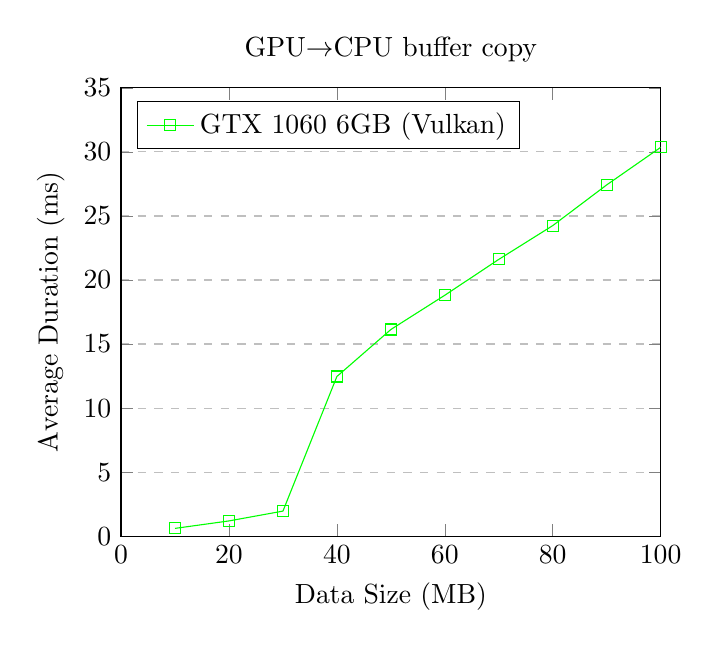
\begin{tikzpicture}
\begin{axis}[
    title={GPU$\rightarrow$CPU buffer copy},
    xlabel={Data Size (MB)},
    ylabel={Average Duration (ms)},
    xmin=0, xmax=100,
    ymin=0, ymax=35,
    xtick={0,20,40,60,80,100},
    ytick={0,5,10,15,20,25,30,35},
    legend pos=north west,
    ymajorgrids=true,
    grid style=dashed,
]

\addplot[color=green, mark=square]
    coordinates {(10.0, 0.608799)(20.0, 1.191449)(30.0, 1.958562)(40.0, 12.465779999999999)(50.0, 16.135205)(60.0, 18.810996)(70.0, 21.609659)(80.0, 24.247859)(90.0, 27.425509)(100.0, 30.35838)};
    \legend{GTX 1060 6GB (Vulkan)}

\end{axis}
\end{tikzpicture}

